\chapter{Introduction}
\label{chap:intro}

%%%%%%%%%%%%%%%%%%%%%%%%%%%%%%%%%%%%%%%%%%%%%%%%%%%%%%%%%%%%%%%%%%%%%%%%%%%%%%%
\section{Background}
\label{sec:chap1-background}

%Intro paragraph\\
%-talk about the increasingly important role of simulation in nuclear?\\
%-challenges for today's nuclear fleet which simulation is well-poised to tackle\\
%-segue into talk about nuclear reactor / neutron physics paragraph\\
%-important to have predictive simulation - needs to be able to extrapolate\\
%-based on empirical models\\
%-complicated core designs, such as the AP1000\\
%-really need to motivate complicated designs since this is relevant to my work\\
%-set the stage for why full-core predictive simulation is needed!!!\\
%-perhaps this is more detail than is necessary for background?\\
%-need to account for angular dependence of neutron flux (e.g. "transport" methods)\\

%\begin{itemize}
%  \item mention advantages of full core transport
%  \begin{itemize}
%    \item optimize core design
%    \item analyze accident-tolerant fuels
%    \item reduce uncertainty magins on CHF
%    \item analysis of advanced non-LWR designs
%  \end{itemize}
%\end{itemize}

Physics simulation has long played an important role in nuclear reactor physics and engineering. The nuclear industry relies on computational modeling of the neutron physics in reactors to predict core reactivity, power distributions, fuel depletion, and transient behavior to ensure the safety and reliability of the current fleet of \ac{LWRs}. Predictive simulations are necessary to evaluate innovations which seek to improve reactor safety and fuel cycle economics, such as reduced safety margin uncertainties, accident-tolerant fuels, and extended cycle lengths. In addition, simulation is used to assess the technical competencies of advanced reactor technologies such as Small Modular Reactors (SMRs), Sodium Fast Reactors (SFRS), Molten Salt Reactors (MSRs), High Temperature Gas Reactors (HTGRs), among other proposed designs. 

Many Generation III+ reactor designs, such as the Westinghouse AP1000\texttrademark \ac{PWR}, optimize performance with complicated core designs. A variety of reactivity control mechanisms -- including partially-inserted control rods, ``grey'' control poisons, \ac{IFBA}, soluble boron, etc. -- along with axial enrichment zoning are used to improve performance metrics such as power peaking factors. The reactor analysis methods in widespread use today assume a ``smoothly'' varying flux distribution, and are not well-suited to model highly localized flux gradients which result from these complex core configurations. New high-fidelity simulation tools are needed to accurately capture neutron physics in advanced reactor designs.

%First paragraph\\
%-wish to replace diffusion with full-core transport\\
%-benefits of improved reactor analysis tools\\
%-HPC may make this possible\\

The nuclear reactor physics community has long strived for whole-core transport-based tools for nuclear reactor analysis. Transport-based methods would enable more accurate core power distributions to be calculated without the approximations needed for today’s tools based upon diffusion theory. Although the computational requirements for full-core transport-based simulations have precluded their widespread development, the continuing growth of cheap parallel processing power has made the prospects for such tools increasingly feasible.

%Second paragraph\\
%-compare contrast competing algorithms - Monte Carlo and deterministic transport\\
%-tradeoff between computational speed/efficiency and accuracy\\
%-crux of deterministic methods are MGXS\\

Core simulation tools utilizing \ac{MC} transport methods represent the ``Holy Grail'' for reactor analysis. However, the computational costs required to accommodate the slow convergence rate for \ac{MC} makes it impractical for widespread use for the foreseeable future. Deterministic transport methods pose a number of advantages to \ac{MC} from a computational perspective, which seems likely to make these methods more viable in the near to intermediate term. However, deterministic methods almost universally discretize the energy domain in a few to hundreds of energy groups. This approximation requires energy condensed \ac{MGXS} in each geometric region to preserve reaction rates. Accurate \emph{reactor agnostic} multi-group cross section generation is needed to enable deterministic transport-based methods to be as accurate and flexible as Monte Carlo in whole-core calculations.

This thesis investigates the potential use of Monte Carlo methods to generate \ac{MGXS} for next-generation whole-core deterministic reactor analyis. Monte Carlo presents a natural approach to replace engineering prescriptions to approximate the flux with a stochastic approximation of the exact flux. The advantage of a \ac{MC}-based approach is that all of the relevant physics modeled in \ac{MC} may be directly embedded into \ac{MGXS}. This improvement in accuracy comes at the computational expense of converging group constant tallies to acceptably low uncertainties. \ac{MC} methods have increasingly been used to generate few group constants for coarse mesh diffusion, most notably by the Serpent \ac{MC} code [CITE]. However, there exist few rigorous and comprehensive analyses of \ac{MGXS} generation from \ac{MGXS} for heterogeneous fine-mesh transport.

The subject matter of this thesis can be organized along two main themes. First, the efficacy of \ac{MGXS} generation with \ac{MC} for fine-mesh transport calculations is rigorously assessed. Some of the approximations made by \ac{MC}-based \ac{MGXS} generation are quantified, including the energy- and spatial-dependence of condensed \ac{MGXS}. An in-depth analysis of systematic bias resulting from constant-in-angle \ac{MGXS} is presented, along with a scheme based on \ac{SPH} factors to compensate for this loss in accuracy. The second theme of this thesis is focused on a new methodology to simultaneously capture local and global spatial self-shielding effects in \ac{MGXS} for whole-core calcuations. This scheme applies statistical clustering to accelerate convergence rate of \ac{MGXS} tallied on high-fidelity spatial meshes in Monte Carlo. The latent variable model which inspires this new scheme is discussed. A series of increasingly complex case studies empirically compare the accuracy and convergence rate of the scheme with traditional \ac{MC}-based MGXS generation.

%Third paragraph\\
%-mention MG would be the reference soln anyway
%-replace deterministic approximation 
%-Existing codes/techniques may not be adequate for full-core transport\\
%-must quantify approximation errors in MGXS for full-core transport \\
%-brief overview of MGXS approximations\\
%-specifically pinpoint angular-dependence and spatial self-shielding\\

Chapter~\ref{chap:intro} motivates the need for new \ac{MGXS} generation techniques with an overview of trends in \ac{HPC} and whole-core transport methods. Chapter~\ref{chap:mgxs} reviews the multi-group cross section approximation, and highlights past efforts to use \ac{MC} to generate \ac{MGXS}. The simulation codes utilized in this thesis are discussed in Chapter~\ref{chap:workflow}, including OpenMC, OpenMOC and OpenCG. The impact of \ac{MGXS} approxmation error is quantified in heterogeneous geometries in Chapter~\ref{chap:biases}. Chapter~\ref{chap:sph} presents an algorithmic approach to address systematic biases resulting from constant-in-angle \ac{MGXS}. A latent variable model for spatial-self shielding effects on \ac{MGXS} is outlined Chapter~\ref{chap:methods}, along with a data pipeline for unsupervised clustering to accelerate the \ac{MGXS} convergence rate. Chapter~\ref{chap:results} evaluates the impact of clustered \ac{MGXS} on the accuracy and convergence rate. Finally, Chapter~\ref{chap:conclusions} summarizes the progress made in this thesis to chart a path forward for \ac{MC}-based \ac{MGXS} generation for whole-core deterministic transport methods.


%%%%%%%%%%%%%%%%%%%%%%%%%%%%%%%%%%%%%%%%%%%%%%%%%%%%%%%%%%%%%%%%%%%%%%%%%%%%%%%
\section{Whole-Core Neutron Transport Simulations}
\label{sec:chap1-whole-core-transport}

\begin{dmath}
\label{eqn:chap1-transport-eqn-6d}
\mathbf{\Omega} \cdot \nabla \Psi(\mathbf{r},\mathbf{\Omega},E) + \Sigma^T(\mathbf{r},E)\Psi(\mathbf{r},\mathbf{\Omega},E) = \int_{0}^{\infty} \mathrm{d}E' \int_{4\pi} \mathrm{d}\mathbf{\Omega'}\Sigma^S(\mathbf{r},{\mathbf{\Omega'}\rightarrow\mathbf{\Omega}},{E'\rightarrow E}) \Psi(\mathbf{r},\mathbf{\Omega'},E') + \frac{\chi(\mathbf{r},E)}{4\pi k_{eff}} \int_{0}^{\infty} \mathrm{d}E' \nu\Sigma^F(\mathbf{r},E') \int_{4\pi} \mathrm{d}\mathbf{\Omega'}\Psi(\mathbf{r},\mathbf{\Omega'},E')
\end{dmath}

Each of the variables in use is defined in \autoref{tab:chap1-variables}. This is a balance equation between neutrons lost to transport, lost to absorption, produced or lost from scattering and those produced from fission. It should be noted that this equation assumes isotropic emission from fission.

\begin{table}[hbt]
  \caption{Variables in the Boltzmann equation.}
  \label{tab:chap1-variables}
  \begin{center}
    \begin{tabular}{ l l }
    \toprule
    Variable & Description \\
    \midrule
    $\mathbf{r}$ & Spatial position vector \\
    $\mathbf{\Omega}$ & Angular direction vector \\
    $E$ & Neutron energy \\
    $\Psi$ & Angular neutron flux \\
    $k_{eff}$ & Effective neutron multiplication factor \\
    $\Sigma^T$ & Neutron total cross section \\
    $\Sigma^S$ & Neutron scattering cross section \\
    $\Sigma^F$ & Neutron fission cross section \\
    $\chi$ & Energy spectrum for fission neutrons \\
    $\nu$ & Average number of neutrons emitted per fission \\
    \bottomrule
  \end{tabular}
  \end{center}
\end{table}

The first step is to simplify this equation by defining those quantities on the right hand side as the total neutron source $Q(\mathbf{r},\mathbf{\Omega},E)$:

\begin{dmath}
\label{eqn:chap1-source}
Q(\mathbf{r},\mathbf{\Omega},E) = \int_{0}^{\infty} \mathrm{d}E' \int_{4\pi} \mathrm{d}\mathbf{\Omega'}\Sigma^S(\mathbf{r},{\mathbf{\Omega'}\rightarrow\mathbf{\Omega}},{E'\rightarrow E}) \Psi(\mathbf{r},\mathbf{\Omega'},E') + \frac{\chi(\mathbf{r},E)}{4\pi k_{eff}} \int_{0}^{\infty} \mathrm{d}E' \int_{4\pi} \mathrm{d}\mathbf{\Omega'} \nu\Sigma^F(\mathbf{r},E')\Psi(\mathbf{r},\mathbf{\Omega'},E')
\end{dmath}

The transport equation can now be more concisely written as follows:

\begin{equation}
\label{eqn:chap1-transport-eqn-src}
\mathbf{\Omega} \cdot \nabla \Psi(\mathbf{r},\mathbf{\Omega},E) + \Sigma^T(\mathbf{r},E)\Psi(\mathbf{r},\mathbf{\Omega},E) = Q(\mathbf{r},\mathbf{\Omega},E)
\end{equation}


%%%%%%%%%%%%%%%%%%%%%%%%%%%%%%%%
\subsection{Monte Carlo Methods}
\label{subsec:chap1-monte-carlo}

\begin{itemize}[noitemsep]
  \item parallel methods (fission bank, DD, multi-threading)
  \item inverse square root convergence rate
  \item poor parallel efficiency - cache unfriendly, difficult to vectorize
  \item impact of correlation on uncertainties
\end{itemize}


%%%%%%%%%%%%%%%%%%%%%%%%%%%%%%%%%%
\subsection{Deterministic Methods}
\label{subsec:chap1-deterministic}


\begin{itemize}[noitemsep]
  \item 2D/1D methods in MPACT, nTracer
  \item Denovo, PDT, 3D OpenMOC, etc.
  \item computational efficiency - cache-friendliness, parallelization, vectorization, etc.
\end{itemize}


%%%%%%%%%%%%%%%%%%%%%%%%%%%%%%%%%%%%%%%%%%%%%%%%%%%%%%%%%%%%%%%%%%%%%%%%%%%%%%%
\section{High-Performance Computing Trends}
\label{sec:chap1-hpc-trends}

first paragraph\\
-parallel computing is making calculations possible for the first time
-
-mention trends of increasing shared memory parallelism

second paragraph\\
-

third paragraph\\
-

\cite{Hunter_Sutton_2013}


%%%%%%%%%%%%%%%%%%%%%%%%%%%%%%%%%%%%%%%%%%%%%%%%%%%%%%%%%%%%%%%%%%%%%%%%%%%%%%%
\section{Multi-Group Cross Sections}
\label{sec:chap1-mgxs}

\begin{itemize}[noitemsep]
  \item black magic ``crux'' of deterministic methods
  \item need accurate \ac{MGXS} for whole core transport methods
  \item motivate \ac{MC} for \ac{MGXS}
  \item must accelerate it in way not possible for conventional \ac{MC}
  \item figure illustrating multi-level approach (see Gibson's thesis)
\end{itemize}

\begin{figure}
%\begin{subfigure}{.5\textwidth}
%  \centering
%  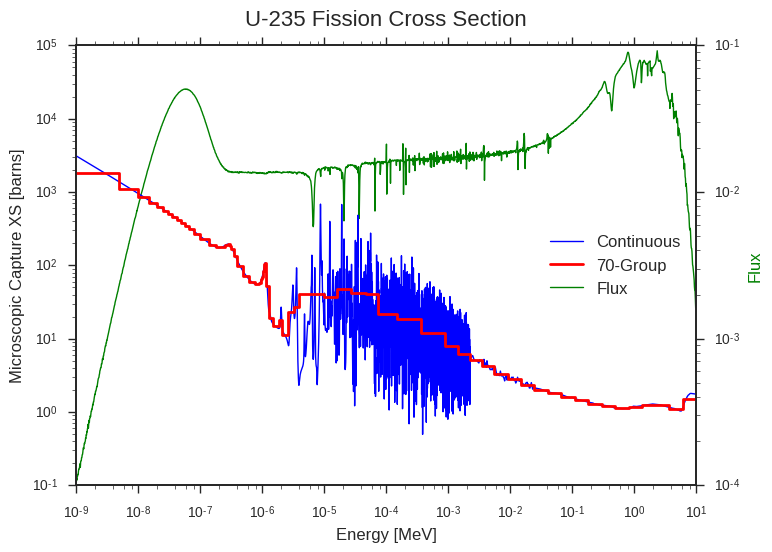
\includegraphics[width=\linewidth]{figures/intro/u235-fission-70}
%  \caption{}
%\end{subfigure}%
\begin{subfigure}{\textwidth}
  \centering
  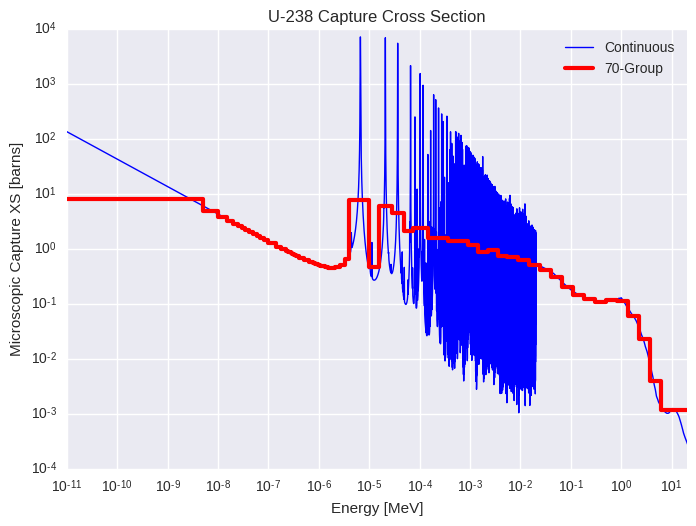
\includegraphics[width=0.9\linewidth]{figures/intro/u238-capture-70}
  \caption{}
\end{subfigure}
%\begin{subfigure}{.5\textwidth}
%  \centering
%  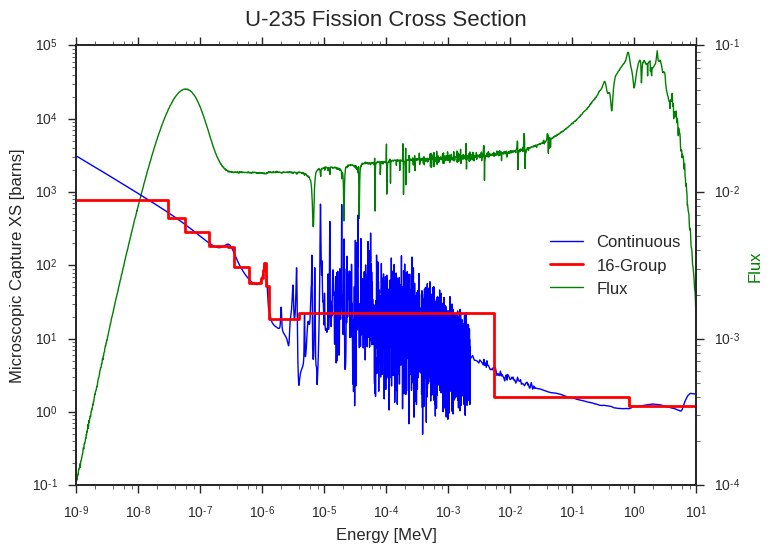
\includegraphics[width=\linewidth]{figures/intro/u235-fission-16}
%  \caption{}
%\end{subfigure}
\begin{subfigure}{\textwidth}
  \centering
  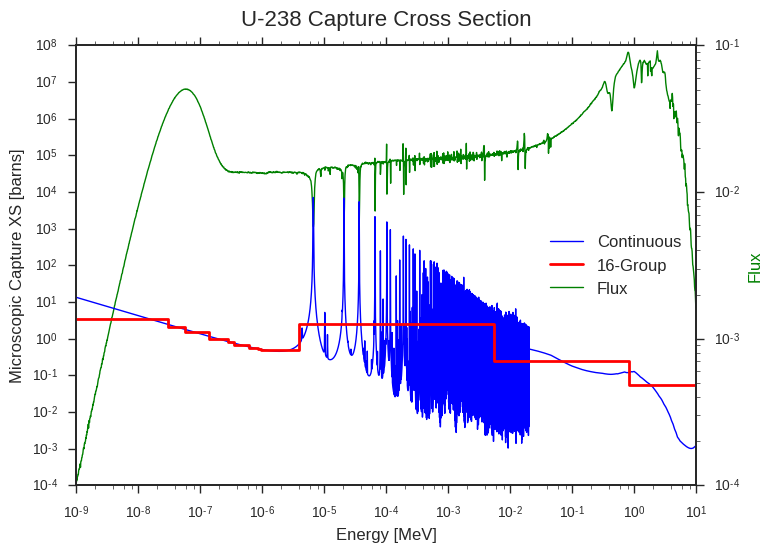
\includegraphics[width=0.9\linewidth]{figures/intro/u238-capture-16}
  \caption{}
\end{subfigure}
%\begin{subfigure}{.5\textwidth}
%  \centering
%  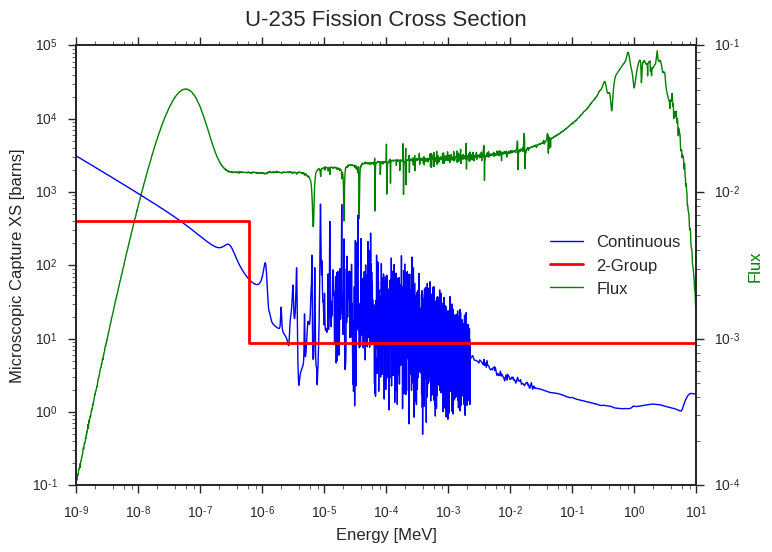
\includegraphics[width=\linewidth]{figures/intro/u235-fission-2}
%  \caption{}
%\end{subfigure}
%\begin{subfigure}{.5\textwidth}
%  \centering
%  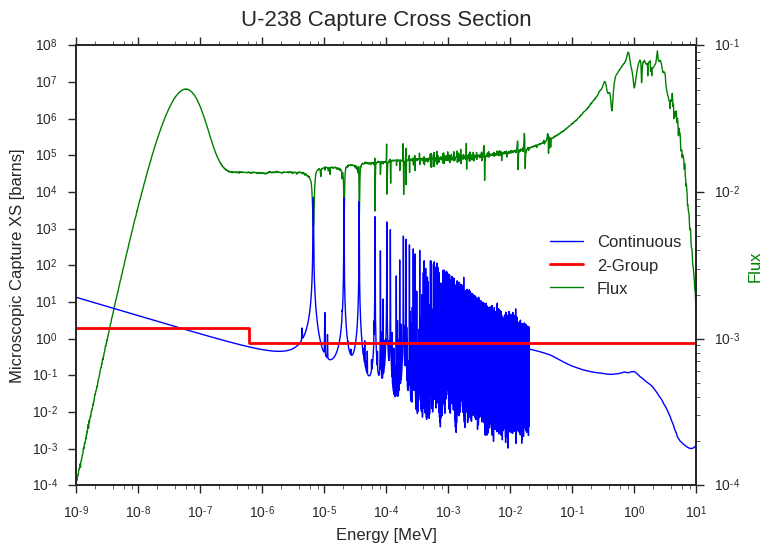
\includegraphics[width=\linewidth]{figures/intro/u238-capture-2}
%  \caption{}
%\end{subfigure}
\caption[Uranium-238 capture cross section]{Continuous energy and multi-group cross sections for U-238 capture in a PWR spectrum for 70-groups (a) and 16-groups (b).}
\label{fig:pwr-ce-mg-xs}
\end{figure}

